%% progress-report-8-SubmapVisualization+ROSPackage tex file.
%% Completed By Yuyang Rong(rongyy@shanghaitech.edu.cn) and
%% Jianxiong Cai(caijx@shanghaitech.edu.cn)
%%
%% To edit this file, please use indentions with tab size of 2.
%%

%% File name unchanged. This is just a temp file.

\documentclass[conference,compsoc]{IEEEtran}
\usepackage{cite}
\usepackage{listings}
\usepackage{blindtext}
\usepackage{enumitem}
% for coding highlight
\usepackage{graphicx}
\usepackage{subfigure}
\usepackage[colorlinks=true,urlcolor=blue]{hyperref}
\usepackage{amsmath, amsthm, amssymb}
\usepackage{subfloat}
\usepackage{ulem}
\usepackage{float}
\usepackage{indentfirst}
\usepackage{color}
\definecolor{codegreen}{rgb}{0,0.6,0}
\definecolor{codegray}{rgb}{0.5,0.5,0.5}
\definecolor{codepurple}{rgb}{0.58,0,0.82}
\definecolor{backcolour}{rgb}{0.95,0.95,0.92}


\lstdefinestyle{mystyle}{
  backgroundcolor=\color{backcolour},   
  commentstyle=\color{codegreen},
  keywordstyle=\color{magenta},
  numberstyle=\tiny\color{codegray},
  stringstyle=\color{codepurple},
  basicstyle=\footnotesize,
  breakatwhitespace=false,         
  breaklines=true,                 
  captionpos=b,                    
  keepspaces=true,                 
  numbers=left,                    
  numbersep=5pt,                  
  showspaces=false,                
  showstringspaces=false,
  showtabs=false,                  
  tabsize=2
}
\lstset{style=mystyle}
\begin{document}
\title{
	Computer Vision Course Project Milestone Report\\
	Gambody \\
}


% author names and affiliations
% use a multiple column layout for up to three different
% affiliations
\author{
	\IEEEauthorblockN{Yuyang Rong, Jingyi Huang, Anqi Pang, Jianxiong Cai, Ziyue Li}
	\IEEEauthorblockA{
		School of Information Science and Technology \\
		ShanghaiTech University \\
	}
}

\maketitle

\begin{abstract}
	In this report we will mark some achievements we have accomplished, and further purpose some problems(along with solutions, maybe) we need to solve in order to reach our goal.
%	In this milestone report we are going to propose the problems we want to solve aiming at our goal of implementing the visual game Gambody. 
	We will specify our technical approach too.
%	We will specify the technical approach we are using at present and what we have achieved so far. The remaining milestones including the dates and sub-goals will be given furthermore.
\end{abstract}
\section{Introduction}
	\par
		We found a popular game called \textit{Hole in the Wall}. In this game one (or two) player(s) are facing a moving wall with a certain shape of hole, the player have to make a specific pose to pass the moving wall or he will be pushed into a water pool behind him.
		Such game is interesting but householders can never have the privilege to play in family gatherings or parties since one can hardly find a moving wall nor adequate safety measurements.
		\begin{figure}[h]
			\centering
			
\includegraphics[width=0.8\linewidth]{./Pic/HIW_Logo}
			\caption{Game Logo}
		\end{figure}
		\begin{figure}[h]
			\centering
			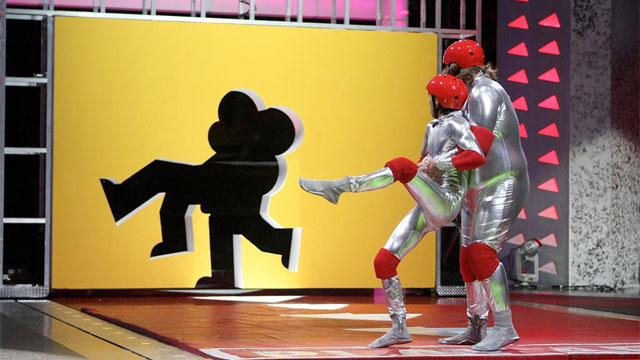
\includegraphics[width=0.45\linewidth]{./Pic/HIW_RedTeam}
			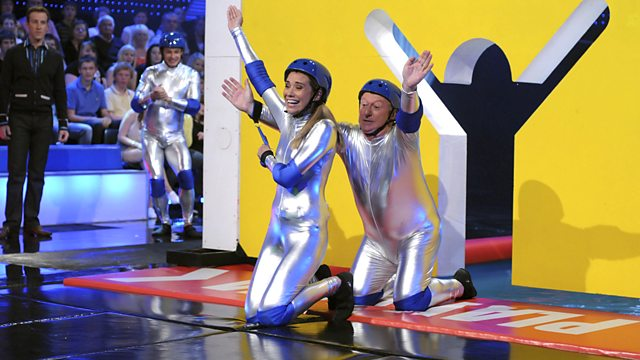
\includegraphics[width=0.45\linewidth]{./Pic/HIW_BlueTeam}
			\caption{Two players in the game posing to pass the wall.}
		\end{figure}
	\par

	\par
		To fix this, we are going to implement a system based on camera so that every one can play this game.
		In our work, we will be using one single camera to track person, it will also give player a bounding box (moving wall).
		The box and player's outfit is compared by our system, the return should be a pass (True) or no pass (False).
%\section{Related Work}
% It seems that this part is not required in the milestone report.
% IF have, please fill in
\section{Technical Approach}
	\subsection{Getting camera stream}
	\par
	We make use of the Image Acquisition Toolbox to connect camera device to MATLAB and achieve real-time image processing and displaying. In general, we keep capturing an image from the camera stream, modify the image we received and show on the screen as long as the camera is working.
	\par
	To be more specific, we first let MATLAB automatically set camera parameters and invoke the camera since the parameters are device dependent. Then a while loop is maintained to implement the primary procedure during the logging time of the camera.
	\par
	One of the obstacle we are facing now is that we can't add some pause time before the result is showed to the player. But it would be best if we give player some time to wait.
	\par
	Also, we need to mirror the image we received, or left and right will be shifted and the user will have a hard time to adapt to it.
	In the first trial we neglected this effect and the game was almost impossible. Now we use a function provided in the MATLAB:
	\begin{lstlisting}[language = MATLAB]
		img = flip(img, 2)\end{lstlisting}
	this function will flip matrix $img$ along the 2nd dimension(row, with column being 1st dimention)
	\subsection{Crop out body}
	\par
	A simple but useful method has been implemented to detect the body. The principle is that given the camera is fixed, the only area has color changing on the image is the body part.
	\par
	In detail, we take a photo of the background first, then we subtract it by the images containing body. As the result, we would get a image with only the body part.
	\begin{figure}[h]
		\centering
		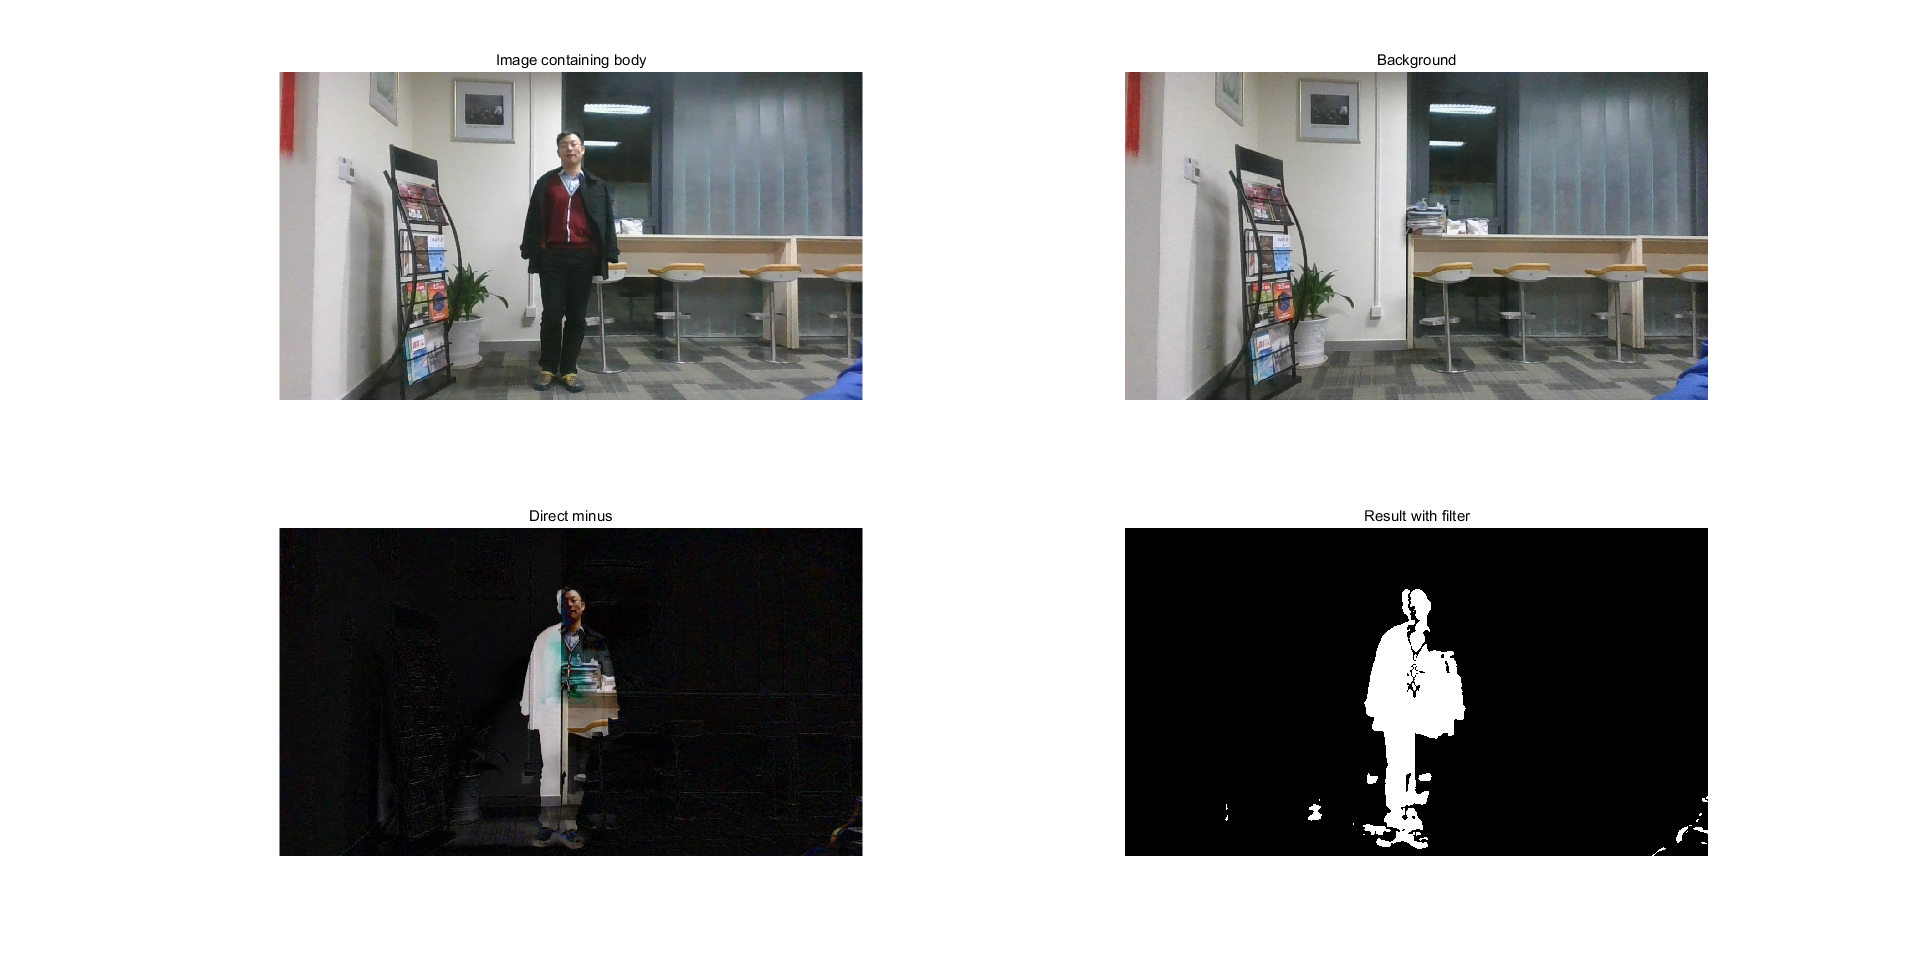
\includegraphics[width=\linewidth]{./Pic/CropBody.png}
		\caption{Upper Left: original photo. Upper Right: Background. Lower Left: the image after subtraction. Lower Right: The body region after we force a threshold. It's clear that only forcing a threshold doesn't work well since shadows, noise will also be counted as part of human body.}
	\end{figure}
	\par
		Due to the noise caused by camera shaking, we use a Gaussian blur and set a threshold to filter out noise. 
		The first version is implemented on the gray value. In other words, the RGB image is first converted to a gray image, doing subtraction, then applying the threshold to get the body.
		Now we are using a threshold of 0.14(gray scale from 0 to 1). 
		Pixels whose gray value are above 0.14 are considered to be part of human body.
	\par
		However, that method brings a problem. Suppose the background is purely green, while the body is purely red. 
		In gray images, they are the same. 
		Thus in the latter version, instead of using the gray image, the body is obtained by comparing RGB raw image. 
		If any of the 3 channel changes a lot, we rule it as part of human body. 
		In the future we will use HSV color space which is more robust to the shadows.
	\par
		After that, there are still some problems, we get some blobs that are not part of the body, and we might lose some part of the body. So we tried to set the largest (and maybe with the second largest) connected binary image to be the crop body.
	\subsection{Generate Masks and Evaluate Results}
		Now that we have get the cropped body from previous part, we can generate masks from it. 
		To reduce the workload of evaluate, we use bonding box to cut the raw image and get a small image which will contain only the body part.
		After that, we set different levels for players so the masks should have their own label of difficult levels.
	\par
		For evaluation part we get two images, one is the players' body and another one is the mask. 
		We normalize the two image so it have robustness for different height and size, then we calculate the correlation of the two pictures and get the biggest correlation value. 
		If the value is bigger than the threshold, then players will pass this level.
		Currently, the threshold is set to 0.95.
	\subsection{Real-time indicator}
	\par
		We need to show the user how he is doing from the image. We considered using words but we determined that it's best to directly show it on the camera feedback.
	\par
		To simultaneously show the mask and the correctness, we decided to change certain channel's value.
		If the player passed, the green channel will be changed, or red channel will. The image will thus be greenish or reddish respectively.
		We will only change pixels in the mask, so the user know what the mask is.
		\begin{figure}[h]
			\centering
			\includegraphics[width=\linewidth]{./Pic/Level}
			\caption{One image in the camera stream. The user knows the result(red means fail, which is the case here) and goal at the same time.}
		\end{figure}	
\section{Remaining Problems}
	\subsection{Body Pose Recognition}
		In our first version of Gambody, we use only binary images to determine whether the player passed or not. 
		A smart player might use the advantage of normalization part and get a pass without a correct pose. 
		Considering this hack, we need body pose recognition from a monocular RGB web-cam.
	\subsection{Background Movement and Multi People}
		We assume background will not move in the first version of our game but reality suggests the otherwise, and maybe there are more than one players. 
		All these will make our assumption fail and so do our code. So we need to deal with multi people and background moving environment.\par
	\subsection{Work To Do}
		To deal with real-time multi-person 2D pose recognition, there are some related works. 
		In our references, there are some methods using CNNs and it is open source. 
		So we decide to use the open source library and rewrite our code by cpp to speed up.\par
		Also to make our work real-time on the household play stations, we can't use pose recognition all the time. So we will estimate the final image and recognize the pose and skeleton to get scores for player.


\bibliographystyle{IEEEtran}
% %% De-comment this line if you have any reference.
% %% And don't forget to change .bib file.
% \bibliography{milestone}
\end{document}
